%%%%%%%%%%%%%%%%%%%%%%%%%%%%%%%%%%%%%%%%%%%%%%%%%%%%%%%%%%%%%%%%%%%%%%%%%%%%%
\chapter{Konzept}
\label{chap:concept}
%%%%%%%%%%%%%%%%%%%%%%%%%%%%%%%%%%%%%%%%%%%%%%%%%%%%%%%%%%%%%%%%%%%%%%%%%%%%%
\chapterstart

Die bestehende Applikation zur Visualisierung und Auflistung von den Ergebnissen der Statischen-Code-Analyse wird als Basis genommen. Um Unterstützungen für das Team bereitstellen zu können, wird die bestehende Applikation und erweitert und weiteres eine Lösung für mobile Geräte entwickelt. Die Daten für das erweiterte Backend und die mobile Applikation kommen aus einer Datenbank, welche mit einem Plugin für verschiedene Projekte befüllt wird.

\section{Bestehende Datenbank und Applikationen}
Das Plugin wird aus der Bachelorarbeit 1 übernommen, die Datenbank um mehrere Tabellen erweitert. Das Plugin wird dazu verwendet, um die Ergebnisse der Statischen Code Analyse in die Datenbank zu importieren. Das Plugin kann in den einzelnen Projekten dazu eingebunden und konfiguriert werden. Die Datenbank ist eine nicht-relationale Lösung. Zu der bestehenden Web-Applikation werden neue Features entwickelt. Um die Funktionalitäten überprüfen zu können, werden mehrere Testprojekte verwendet. 

\section{Funktionalitäten}
\subsection{Webapplikation}
Um eine Teamfunktion integrieren zu können und damit die Code Qualität steigern zu können, muss eine Userverwaltung hinzugefügt werden. User müssen sich registrieren und anmelden können. Ebenso muss eine Team- und Projektverwaltung implementiert werden. Hierbei muss auch die Rechteverwaltung beachtet werden, da zum Beispiel nur Teammitglieder Projektdaten sehen dürfen und nur ausgewählte Benutzerinnen und Benutzer auf ein Projekt zugriff haben dürfen. Um die einzelnen Fehler und Bugs zuordnen zu können, muss eine Interaktion mit einem Programm für die Versionsverwaltung implementiert werden. Über diese Versionsverwaltung kann unter anderem festgestellt werden, welche Teammitglieder welche Bugs implementiert haben. Die Darstellungen sollen hierbei genau den entsprechenden Code auflisten. Weitere Funktionalitäten und Features soll ein automatisch generierte Fehlerreport für das Team sein, der auch automatisch versendet werden soll. Da eine eigene Benutzerverwaltung eingebaut wird, eignet sich die Webapplikation gut für die Installierung auf einem eigenen Server der Firma.
\subsection{Mobile Applikation}
In der mobilen Applikation sollen die wichtigsten Daten der Webapplikation einfach und übersichtlich aufbereitet werden. Die Daten kommen hierbei von der Webapplikation, da eine eigene Datenbank zu viele Ressourcen verbrauchen würde. Eine mobile Lösung bietet den Vorteil, dass die Inhalte überall angesehen werden können. Ein wichtiger Aspekt ist hierbei die Interaktion einer Art spielerischen Funktion, da diese das Interesse der Benutzerinnen und Benutzer an der Applikation verstärken könnte. Ein weiterer wichtiger Aspekt ist die Darstellung, da die Daten kompakt angezeigt werden müssen. Werden zu viele Daten angezeigt, können sich die Benutzerinnen und Benutzer mit der Fülle an Daten überfordert fühlen. 

\section{Infrastruktur und Interaktion der Teilprojekte}
Mehrere Applikationen und Systeme werden für die Arbeit verwendet (siehe Abbildung 3.1): \\
Das \textit{Project} ist das Softwareprojekt, welches analysiert und auf Fehler in der Code Qualität untersucht werden soll. Diese Daten werden mithilfe des \textit{Plugin} in die Datenbank importiert und dort gespeichert. Weiteres werden in der Datenbank die Einstellungen für die einzelnen Projekte und die User gespeichert. Das \textit{Backend} liest die Daten aus und bereitet sie für die Analyse im Frontend vor. Das Backend kontrolliert auch die Berechtigungszugriffe und die Berichte für die Teams. In der \textit{Weboberfläche} werden die Informationen angezeigt, welche aus dem Backend abgefragt werden. Um Zugriff zur Weboberfläche zu bekommen, muss die Benutzerin oder der Benutzer sich anmelden. Die Benutzerdaten werden in der Datenbank gespeichert.
Die \textit{Mobile Applikation} bekommt die Daten aus dem Backend und zeigt sie an. Wird im \textit{Project} eine Versionsverwaltung verwendet, so kann das in der \textit{Weboberfläche} angegeben werden. Ist dies der Fall, so kann das Backend Daten aus dem Tool der Versionsverwaltung bekommen. (Informationen zu Commits, Benutzerinnen und Benutzer, veränderte und neue Files). Diese Daten werden daraufhin im Backend wieder aufbereitet und in der Weboberfläche den entsprechenden Teammitgliedern angezeigt.
\begin{figure}[tp]
  \centering
  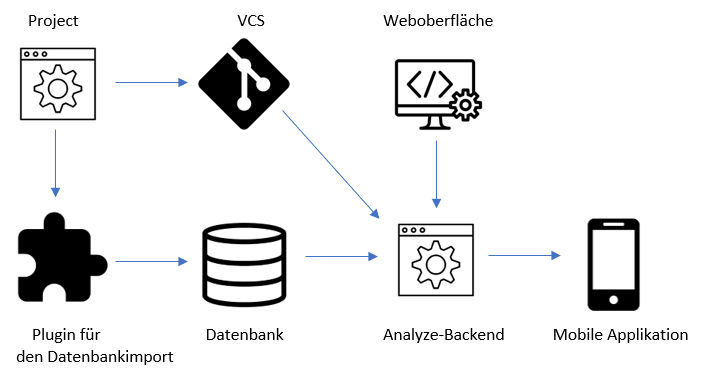
\includegraphics[height=8cm]{images/infrastruktur.PNG}
  % The short caption should be capitalised
  % The full caption should hold a full sentence. 
 \caption[Infrastruktur und beteiligte Applikationen und Systeme]{Infrastruktur sowie beteiligte Applikationen und Systeme. Die Pfeile zeigen hierbei den Datenfluss zwischen den einzelnen Systemen und Applikationen an.}
  \label{fig:findingsInIDE}
\end{figure}
\\ \\ Das hier beschriebene Konzept beinhaltet die zu entwickelnden Funktionalitäten und Überlegungen zu Infrastruktur und Projekt, stellt aber nicht die eigentliche Lösung da. Dies wird in Kapitel 4, Umsetzung, beschrieben.
\chapterend